\documentclass[aspectratio=169,10pt]{beamer}

\usetheme{Madrid}
\usecolortheme{default}
\setbeamertemplate{navigation symbols}{}
\setbeamertemplate{footline}[frame number]
\ifdefined\showNotes
  \setbeameroption{show notes on second screen=right}
\else
  \setbeameroption{hide notes}
\fi
\setbeamersize{text margin left=8mm,text margin right=8mm}
\setbeamertemplate{itemize item}{\color{positive}\scriptsize\raisebox{0.15ex}{\textbullet}}
\setbeamertemplate{itemize subitem}{\color{emphasis}\scriptsize\raisebox{0.15ex}{\textbullet}}

\usepackage{amsmath,amssymb,booktabs,mathtools}
\usepackage{graphicx}
\usepackage{hyperref}
\usepackage{tikz}
\usetikzlibrary{arrows.meta,positioning,calc}
\usepackage{tabularx}
\usepackage{ragged2e}
\usepackage{xcolor}
\usepackage{xeCJK}
\setCJKmainfont{FandolSong-Regular.otf}
\setCJKsansfont{FandolHei-Regular.otf}
\setCJKmonofont{FandolFang-Regular.otf}

\definecolor{positive}{HTML}{005A8D}
\definecolor{negative}{HTML}{9A5A00}
\definecolor{emphasis}{HTML}{007A5A}
\definecolor{neutral}{HTML}{4B5563}
\definecolor{cbPurple}{HTML}{7A3E76}
\definecolor{ink}{HTML}{1F2937}
\definecolor{softblue}{HTML}{EAF3F8}
\definecolor{softgreen}{HTML}{EAF7F2}
\definecolor{softorange}{HTML}{FFF4E5}

\newcommand{\pos}[1]{\textcolor{positive}{#1}}
\newcommand{\con}[1]{\textcolor{negative}{#1}}
\newcommand{\HL}[1]{\textcolor{emphasis}{#1}}
\newcommand{\muted}[1]{\textcolor{neutral}{#1}}
\newcommand{\LLMAgg}{\textsf{LLMAgg}}
\newcommand{\FactOWL}{\textsf{FactOWL}}
\newcommand{\RiDiC}{\textsf{RiDiC}}
\newcommand{\Kfull}{K_{\mathrm{full}}}
\pdfstringdefDisableCommands{\def\\{, }\def\and{; }\def\translate#1{}}

\setbeamercolor{normal text}{fg=ink,bg=white}
\setbeamercolor{structure}{fg=positive}
\setbeamercolor{frametitle}{fg=ink,bg=white}
\setbeamercolor{title}{fg=white}
\setbeamercolor{subtitle}{fg=white}
\setbeamercolor{author in head/foot}{fg=neutral}
\setbeamercolor{block title alerted}{fg=white,bg=negative}
\setbeamercolor{block body alerted}{fg=ink,bg=softorange}
\setbeamercolor{date in head/foot}{fg=neutral}

\title[Adaptive Self-Consistency]{Adaptive Self-Consistency for Long-Form Factuality on Long-Tail Facts}
\subtitle{Aggregation, metric sensitivity, and audited budget routing}
\author[D. Moskovskiy et al.]{Daniil Moskovskiy \and Rafael Grigoryan \and Evgenii Shuranov \\ Wenshuai Yin \and Alexander Panchenko}
\institute{AIRI \textbullet\ Skoltech \textbullet\ MSU \textbullet\ ITMO University \textbullet\ HSE}
\date{KONVENS 2026}
\hypersetup{
  pdftitle={Adaptive Self-Consistency for Long-Form Factuality on Long-Tail Facts},
  pdfauthor={Daniil Moskovskiy et al.},
  pdfsubject={LLM aggregation and adaptive inference for long-form factuality}
}

\begin{document}

\begin{frame}[plain]
  \titlepage
  \note{Key message: aggregation can improve the executed factuality score, but the metric and budget evaluation require careful interpretation. Transition: first define the empirical questions and the audited evaluation.}
\end{frame}

\begin{frame}{Fluent long answers can hide many factual failures}
  \begin{columns}[T,onlytextwidth]
    \column{0.47\textwidth}
      \begin{block}{The setting}
        \begin{itemize}
          \item Entity-centric questions require \textbf{long, coherent answers}.
          \item Each answer contains many independently checkable claims.
          \item Rare entities make parametric recall less reliable.
        \end{itemize}
      \end{block}
      \vspace{4pt}
      \centering
      {\large \textbf{Fluency} $\neq$ \textbf{factual precision}}
    \column{0.47\textwidth}
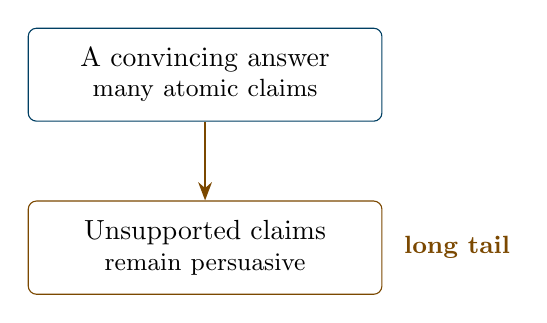
\begin{tikzpicture}[x=1cm,y=1cm]
  \node[draw=positive!70!black,fill=white,rounded corners=3pt,
        text width=4.0cm,align=center,inner sep=7pt] (answer)
        {A convincing answer\\[-1pt]{\small many atomic claims}};
  \node[draw=negative!80!black,fill=white,rounded corners=3pt,
        text width=4.0cm,align=center,inner sep=7pt,below=1.0cm of answer] (risk)
        {Unsupported claims\\[-1pt]{\small remain persuasive}};
        \draw[-{Stealth},thick,negative!80!black] (answer) -- (risk);
        \node[font=\small\bfseries,negative!80!black,right=0.15cm of risk] {long tail};
      \end{tikzpicture}
  \end{columns}
  \vspace{5pt}
  \begin{alertblock}{Core tension}
    More samples can reveal correct facts. A fixed large budget still wastes compute after gains level off.
  \end{alertblock}
  \note{Key message: the paper treats factuality as a claim-level problem and compute as a variable resource. Transition: this motivates three empirical questions rather than a new evaluator or benchmark.}
\end{frame}

\begin{frame}{Three questions organize the study}
  \begin{columns}[T,onlytextwidth]
  \color{ink}
    \column{0.30\textwidth}
      \centering
      {\color{positive}\fontsize{34}{38}\selectfont 1}\par\vspace{2pt}
      \textbf{Does sampling help?}\par\vspace{3pt}
      \small Across head, torso, and tail entities.
    \column{0.30\textwidth}
      \centering
      {\color{emphasis}\fontsize{34}{38}\selectfont 2}\par\vspace{2pt}
      \textbf{How should candidates combine?}\par\vspace{3pt}
      \small Synthesis versus voting and selection.
    \column{0.30\textwidth}
      \centering
      {\color{negative}\fontsize{34}{38}\selectfont 3}\par\vspace{2pt}
      \textbf{Can compute be routed?}\par\vspace{3pt}
      \small Preserve factuality while reducing samples.
  \end{columns}
  \vfill
  \begin{block}{Empirical thesis}
    \centering
    \large \LLMAgg{} improves the executed \FactOWL{} score; budget conclusions depend on the metric, and adaptive routing remains exploratory.
  \end{block}
  \note{Key message: keep the talk focused on these three questions. Transition: answer them with a controlled multilingual, multi-domain evaluation.}
\end{frame}

\begin{frame}{Evaluation: LLM-judged FactOWL score across tiers}
  \begin{columns}[T,onlytextwidth]
    \column{0.48\textwidth}
      \begin{block}{\RiDiC{} benchmark}
        \begin{itemize}
          \item 3 domains: rivers, cars, disasters.
          \item 2 languages: English and Chinese.
          \item Wikipedia pageview tiers: \textbf{head}, torso, \textbf{tail}.
          \item Public pool: up to 99 completions per input.
        \end{itemize}
      \end{block}
      \vspace{4pt}
      \centering
      \textbf{Same generator:} Llama 3.1 8B Instruct
    \column{0.47\textwidth}
      \begin{block}{Reported score ($\gamma=10$)}
        \small
        \begin{align*}
          p(y) &= \frac{1}{n}\sum_{i=1}^{n}\mathbf{1}[f_i\ \text{supported}],\\[-2pt]
          S_{10}(y) &= p(y)\!\begin{cases}
            1, & n>10,\\
            \exp(1-10/n), & n\leq 10.
          \end{cases}
        \end{align*}
        \scriptsize Atomic facts and support labels are LLM-judged against the supplied Wikipedia page. For $n=0$, $S_{10}(y)=0$.
      \end{block}
  \end{columns}
  \vspace{0pt}
  \begin{center}
    \color{ink}
    \footnotesize
    \renewcommand{\arraystretch}{0.75}
    \begin{tabular}{@{}llll@{}}
      \toprule
      \textbf{Lang.} & \textbf{Domain} & \textbf{Tier} & \textbf{RiDiC entity example}\\
      \midrule
      EN & cars      & tail  & Jiotto Caspita\\
      EN & rivers    & head  & Blue Nile\\
      EN & disasters & torso & Super Outbreak\\
      ZH & cars      & tail  & 劳斯莱斯 Silver Wraith\\
      ZH & disasters & torso & 2024年花蓮地震\\
      ZH & rivers    & head  & 伏尔塔瓦河\\
      \bottomrule
    \end{tabular}
  \end{center}
  \note{Key message: all headline tables use the executed gamma-10 score, not plain factual precision. Fact extraction and support verification are model-judged proxies grounded in the supplied page. Transition: now show where sampling and synthesis enter the pipeline.}
\end{frame}

\begin{frame}{Method: sample, synthesize, score, then route the budget}
  \centering
  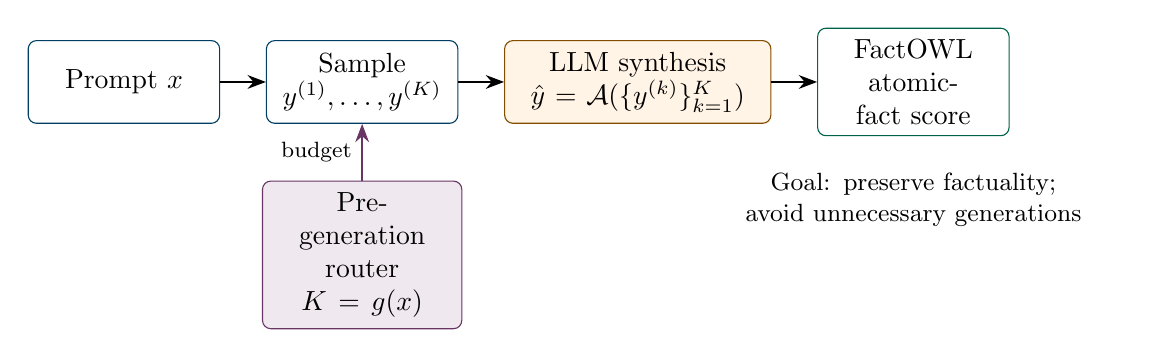
\begin{tikzpicture}[
      >=Stealth,
      node distance=0.72cm and 0.58cm,
      box/.style={draw=positive!70!black,fill=white,rounded corners=3pt,
                  minimum height=1.05cm,text width=2.15cm,align=center,inner sep=4pt},
      agg/.style={box,draw=negative!85!black,fill=softorange,text width=3.1cm},
      score/.style={box,draw=emphasis!80!black,fill=white,text width=2.15cm},
      route/.style={draw=cbPurple!85!black,fill=cbPurple!12,rounded corners=3pt,
                    text width=2.25cm,align=center,inner sep=4pt}
    ]
    \node[box] (input) {Prompt $x$};
    \node[box,right=of input] (sample) {Sample\\$y^{(1)},\ldots,y^{(K)}$};
    \node[agg,right=of sample] (aggregate) {LLM synthesis\\$\hat y=\mathcal{A}(\{y^{(k)}\}_{k=1}^{K})$};
    \node[score,right=of aggregate] (fact) {FactOWL\\atomic-fact score};
    \node[route,below=0.72cm of sample] (adaptive) {Pre-generation\\router $K=g(x)$};
    \draw[->,thick] (input) -- (sample);
    \draw[->,thick] (sample) -- (aggregate);
    \draw[->,thick] (aggregate) -- (fact);
    \draw[->,thick,draw=cbPurple!85!black] (adaptive) -- node[left,font=\footnotesize] {budget} (sample);
    \node[font=\small,align=center,text width=5.2cm,below=0.35cm of fact] {Goal: preserve factuality; avoid unnecessary generations};
  \end{tikzpicture}
  \vfill
  \begin{itemize}
    \item \textbf{Single:} candidate 1 from the same fixed pool.
    \item \textbf{LLMAgg:} merge consistent claims and remove contradictions.
    \item \textbf{Adaptive:} exploratory pre-generation choice of $K$.
  \end{itemize}
  \note{Key message: the intervention is content-level synthesis plus a separate pre-generation budget policy. Transition: why synthesis matters becomes clearer when candidate answers disagree.}
\end{frame}

\begin{frame}{Synthesis has two distinct regimes}
  \begin{columns}[T,onlytextwidth]
    \column{0.47\textwidth}
      \begin{block}{Complementary evidence}
        \begin{itemize}
          \item Correct claims distributed across candidates.
          \item Agreement helps recover a shared core.
          \item Synthesis can exceed every input response.
        \end{itemize}
      \end{block}
    \column{0.47\textwidth}
      \begin{alertblock}{Correlated error}
        \begin{itemize}
          \item Candidates repeat related false claims.
          \item Agreement is not evidence of truth.
          \item Aggregation can amplify the wrong signal.
        \end{itemize}
      \end{alertblock}
  \end{columns}
  \vfill
  \centering
  \large Selection inherits one response; \LLMAgg{} constructs a new response from the pool.
  \note{Key message: synthesis helps only when the pool contains recoverable complementary evidence. Correlated errors create the opposite regime, so agreement alone is not a safety guarantee. Transition: compare the mechanisms explicitly.}
\end{frame}

\begin{frame}{Baselines separate agreement, selection, and synthesis}
  \begin{center}
  \color{ink}
  \begin{tabularx}{0.94\textwidth}{@{}l X l@{}}
    \toprule
    \textbf{Condition} & \textbf{What it does} & \textbf{Deployable?}\\
    \midrule
    Single & First completion from the same fixed pool & yes\\
    MC & Majority co-occurrence over responses & yes\\
    MF & Majority voting over normalized atomic facts & yes\\
    Best-of-$K$ logprob & Same selector on the matched $K=20$ pool & yes\\
    Best sampled & Oracle picks factuality-best candidate after scoring & no\\
    \LLMAgg{} & LLM synthesizes a new response from the pool & yes\\
    \bottomrule
  \end{tabularx}
  \end{center}
  \vspace{8pt}
  \begin{block}{Fair comparison}
    \small Single is candidate 1 of the shared pool. Matched-$K$ methods use the same first 20 candidates; full-budget results use all 99.
  \end{block}
  \note{Key message: the paper does not compare one vague baseline against one vague method; it isolates response agreement, fact voting, logprob selection, oracle selection, and content synthesis. Transition: the main table shows a consistent ordering.}
\end{frame}

\begin{frame}{At matched $K=20$, synthesis leads selection baselines}
  \begin{center}
  \vspace{4pt}
  \color{ink}
  \begin{tabular}{@{}lrrrr@{}}
    \toprule
    & \textbf{Single} & \textbf{Best-of-$K$} & \textbf{ReASC} & \textbf{\LLMAgg{}@20}\\
    \midrule
    English macro & 0.281 & 0.304 & 0.290 & \textbf{\pos{0.577}}\\
    Chinese macro & 0.324 & 0.375 & 0.331 & \textbf{\pos{0.564}}\\
    \bottomrule
  \end{tabular}
  \end{center}
  \vspace{8pt}
  \begin{columns}[T,onlytextwidth]
    \column{0.47\textwidth}
      \begin{block}{Across six language--domain cells}
        \begin{itemize}
          \item Same first-20 candidate pool.
          \item \LLMAgg{} leads both selection policies.
          \item Gains are broad, not driven by one domain.
        \end{itemize}
      \end{block}
    \column{0.47\textwidth}
      \begin{alertblock}{Interpretation}
        \small These are executed $S_{10}$ scores; they are not plain supported-fact precision.
      \end{alertblock}
  \end{columns}
  \note{Key message: this is a strictly compute-matched comparison over the same first 20 candidates. LLMAgg reaches 0.577 in English and 0.564 in Chinese, ahead of the first candidate, log-probability selection, and corrected ReASC. Values use the executed gamma-10 score. Transition: quantify how the apparent budget threshold changes with the metric.}
\end{frame}

\begin{frame}{Operational $K$ thresholds depend on the metric}
  \begin{columns}[T,onlytextwidth]
    \column{0.47\textwidth}
      \begin{block}{Executed $S_{10}$: $K_{95}/K_{99}$}
        \centering\small
        \begin{tabular}{@{}lrr@{}}
          \toprule
          & EN & ZH\\
          \midrule
          Cars      & 4/8  & 8/16\\
          Disasters & 8/20 & 8/16\\
          Rivers    & 8/16 & 8/16\\
          \bottomrule
        \end{tabular}
      \end{block}
    \column{0.47\textwidth}
      \begin{alertblock}{Raw support $p(y)$: $K_{95}/K_{99}$}
        \centering\small
        \begin{tabular}{@{}lrr@{}}
          \toprule
          & EN & ZH\\
          \midrule
          Cars      & 1/1 & 1/8\\
          Disasters & 1/1 & 2/4\\
          Rivers    & 1/1 & 4/16\\
          \bottomrule
        \end{tabular}
      \end{alertblock}
  \end{columns}
  \vfill
  \centering
  \small $K_q$: earliest tested $K\in\{1,2,4,8,16,20\}$ reaching $q\%$ of the $K=20$ score. No formal $K_{\mathrm{sat}}$ is estimated.
  \note{Key message: the earlier claim of saturation around K=8--16 was metric-dependent. Under the executed gamma-10 score those are useful operational thresholds; under plain supported-fact precision, English reaches the K20 level at K1. Transition: popularity remains a separate structural axis.}
\end{frame}

\begin{frame}{Aggregation improves tail entities, but the head-to-tail gap remains}
  \begin{center}
  \small
  \color{ink}
  \begin{tabular}{@{}llrrrr@{}}
    \toprule
    & & \multicolumn{2}{c}{\textbf{Single}} & \multicolumn{2}{c}{\textbf{LLMAgg@20}}\\
    \textbf{Lang.} & \textbf{Tier} & \multicolumn{2}{c}{macro $S_{10}$} & \multicolumn{2}{c}{macro $S_{10}$}\\
    \midrule
    EN & head  & \muted{0.445} & & \pos{0.828} & \\
    EN & torso & \muted{0.384} & & \pos{0.762} & \\
    EN & tail  & \muted{0.243} & & \pos{0.513} & \\
    \midrule
    ZH & head  & \muted{0.480} & & \pos{0.757} & \\
    ZH & torso & \muted{0.396} & & \pos{0.675} & \\
    ZH & tail  & \muted{0.275} & & \pos{0.501} & \\
    \bottomrule
  \end{tabular}
  \end{center}
  \vspace{7pt}
  \begin{columns}[T,onlytextwidth]
    \column{0.47\textwidth}
      \begin{block}{Stable pattern}\small
        Head $>$ torso $>$ tail remains visible after improved inference.
      \end{block}
    \column{0.47\textwidth}
      \begin{alertblock}{Implication}\small
        Aggregation raises executed score broadly; long-tail difficulty remains.
      \end{alertblock}
  \end{columns}
  \vspace{3pt}
  \centering
  {\footnotesize Single is candidate 1 from the shared pool; values are macro averages over three domains.}
  \note{Key message: on the executed gamma-10 score, LLMAgg improves every popularity tier but does not erase the head--tail gap. This is not a claim about an independently sampled Single. Transition: audit the adaptive-budget evidence.}
\end{frame}

\begin{frame}{The original $K=99$ controller is not held-out evidence}
  \begin{columns}[T,onlytextwidth]
    \column{0.47\textwidth}
      \begin{alertblock}{Audit findings}
        \begin{itemize}
          \item Eight baseline rows created per topic.
          \item Split performed row-wise, not by topic.
          \item Nearly every test topic appears in training.
          \item Raw score joins duplicate repeated titles.
        \end{itemize}
      \end{alertblock}
    \column{0.47\textwidth}
      \begin{block}{Consequences}
        \begin{itemize}
          \item Feature importance is not interpretable.
          \item Bootstrap rows are not independent.
          \item Reported $>99\%$ retention is not a generalization result.
          \item Savings of 2--29\% remain descriptive only.
        \end{itemize}
      \end{block}
  \end{columns}
  \vfill
  \centering
  \textbf{The adaptive headline is withdrawn pending a topic-grouped rerun.}
  \note{Key message: post-audit, the original K99 controller cannot support a held-out routing claim. The leakage comes from expanding each topic over baseline K values before a row-wise split. Transition: deduplicated K20-targeted recomputations give a more informative negative result.}
\end{frame}

\begin{frame}{Deduplicated $K=20$ reruns save compute but miss targets}
  \begin{columns}[T,onlytextwidth]
    \column{0.47\textwidth}
      \begin{block}{Observed range}
        \begin{itemize}
          \item Average $K$: \textbf{6.1--8.9}.
          \item Generation savings: \textbf{56--70\%}.
          \item Score retention: \textbf{0.85--0.88}.
          \item Target coverage: \textbf{0.40--0.52}.
        \end{itemize}
      \end{block}
    \column{0.47\textwidth}
      \begin{alertblock}{Why a range?}
        \begin{itemize}
          \item Repeated titles have conflicting saved scores.
          \item Keep-first versus keep-last changes exact cells.
          \item Zero-score baselines make ratios undefined.
          \item The negative conclusion is unchanged.
        \end{itemize}
      \end{alertblock}
  \end{columns}
  \vfill
  \centering
  \textbf{Compute falls, but the requested 0.95/0.99 retention is not achieved.}
  \note{Key message: after enforcing unique topics and one-to-one score joins, K20-targeted reruns use roughly six to nine samples and save 56--70 percent. Exact cells vary with duplicate resolution, but retention stays around 0.85--0.88 and only 40--52 percent of nonzero-baseline examples meet target. Transition: separate what remains supported from what is still open.}
\end{frame}

\begin{frame}{Adaptive routing remains an open problem}
  \begin{columns}[T,onlytextwidth]
    \column{0.47\textwidth}
      \begin{block}{Supported after audit}
        \begin{itemize}
          \item Deduplicated reruns reduce average $K$.
          \item Some topics benefit substantially beyond $K=20$.
          \item Example: Debby, $0.000\to0.622$ from $K=20\to99$.
        \end{itemize}
      \end{block}
      \vspace{5pt}
      \centering
      \textbf{Per-topic curves are non-monotonic.}
    \column{0.47\textwidth}
      \begin{alertblock}{Not supported}
        \begin{itemize}
          \item Reliable 0.95/0.99 retention.
          \item Generalization of the $K=99$ policy.
          \item Detection of aggregation failures.
          \item A universal saturation budget.
        \end{itemize}
      \end{alertblock}
      \vspace{5pt}
      \centering
      \textbf{Use grouped splits and explicit zero handling.}
  \end{columns}
  \note{Key message: the current evidence supports only an exploratory routing result. Large per-topic gains beyond K20 exist, but the tested features do not reliably identify them. A valid rerun must split by topic, enforce unique score keys, and define zero-baseline behavior before evaluation. Transition: close with the claims that survive the audit.}
\end{frame}

\begin{frame}{Three takeaways}
  \begin{enumerate}
    \item \textbf{Synthesis leads on the executed $S_{10}$ score.}\\
          \small Single is candidate 1 from the same fixed pool.
    \vspace{6pt}
    \item \textbf{Budget thresholds are metric-dependent.}\\
          \small No formal or universal $K_{\mathrm{sat}}$ is established.
    \vspace{6pt}
    \item \textbf{Adaptive routing is not yet validated.}\\
          \small Deduplicated K20 reruns save compute but miss retention targets.
  \end{enumerate}
  \vfill
  \begin{block}{Answer to the opening tension}
    \centering
    \large Aggregation can help; efficient routing requires leakage-free evaluation.
  \end{block}
  \note{Key message: distinguish the executed score from raw factual precision, treat K thresholds as operational and metric-specific, and do not present the original adaptive controller as held-out evidence. Transition: references, then questions.}
\end{frame}

\begin{frame}{References}
  \small
  \begin{thebibliography}{9}
    \bibitem{paper}
      D. Moskovskiy et al.\newblock Adaptive Self-Consistency for Long-Form Factuality on Long-Tail Facts. 2026.
    \bibitem{ridic}
      P. Braslavski et al.\newblock The Chronicles of RiDiC: Generating Datasets with Controlled Popularity Distribution for Long-form Factuality Evaluation. 2026.
    \bibitem{sc}
      X. Wang et al.\newblock Self-Consistency Improves Chain of Thought Reasoning in Language Models. ICLR, 2023.
    \bibitem{reasc}
      J. Kim et al.\newblock Reliability-Aware Adaptive Self-Consistency for Efficient Sampling in LLM Reasoning. ACL Findings, 2026.
    \bibitem{factowl}
      A. Sakhovskiy et al.\newblock FactOWL: A Cost-Efficient Tool for Long-Form Factuality Evaluation. SIGIR, 2026.
  \end{thebibliography}
  \note{Key message: the primary paper builds on self-consistency and fact-level factuality evaluation, but studies their interaction under long-tail and budget constraints. Transition: thank the audience and invite questions.}
\end{frame}

\begin{frame}{Thank you}
  \color{ink}
  \begin{center}
    \vspace{1.5cm}
    {\Huge\bfseries Questions?}\\[14pt]
    {\normalsize\texttt{Daniil Moskovskiy \textbar{} A.Panchenko@skol.tech}}
  \end{center}
  \note{Close: aggregation improves the executed score, while metric sensitivity and adaptive-budget validation remain open. Invite questions about the audit, evaluator reliability, and per-topic non-monotonicity.}
\end{frame}

\appendix

\begin{frame}{Backup slides}
  \color{ink}
  \begin{center}
    \vspace{1.5cm}
    {\Huge\bfseries Backup slides}\\[8pt]
    {\large Audited tables, definitions, and case traces}
  \end{center}
  \note{Use these slides for questions about exact per-cell values, policy definitions, dataset filtering, or qualitative behavior.}
\end{frame}

\begin{frame}{Matched-$K=20$ comparison by language and domain}
  \small
  \begin{center}
  \color{ink}
  \begin{tabular}{@{}llrrr@{}}
    \toprule
    \textbf{Lang.} & \textbf{Domain} & \textbf{Single} & \textbf{LLMAgg@20} & \textbf{Gain}\\
    \midrule
    EN & rivers    & 0.211 & 0.463 & +0.252\\
    EN & cars      & 0.344 & 0.655 & +0.311\\
    EN & disasters & 0.287 & 0.612 & +0.325\\
    \midrule
    ZH & rivers    & 0.269 & 0.442 & +0.173\\
    ZH & cars      & 0.349 & 0.633 & +0.285\\
    ZH & disasters & 0.354 & 0.616 & +0.262\\
    \bottomrule
  \end{tabular}
  \end{center}
  \vspace{8pt}
  \begin{block}{Reading the table}
    \small Values use executed $S_{10}$ on the same matched subset. Single is candidate 1 from the first-20 pool.
  \end{block}
  \note{Use this slide to answer questions about individual cells behind the macro averages.}
\end{frame}
\begin{frame}{Supplementary baselines at matched $K=20$}
  \small
  \begin{center}
  \color{ink}
  \begin{tabular}{@{}llrrrr@{}}
    \toprule
    \textbf{Lang.} & \textbf{Domain} & \textbf{Single} & \textbf{Best-of-$K$ logprob} & \textbf{ReASC} & \textbf{\LLMAgg{}@20}\\
    \midrule
    EN & cars      & 0.344 & 0.366 & 0.354 & 0.655\\
    EN & disasters & 0.287 & 0.324 & 0.305 & 0.612\\
    EN & rivers    & 0.211 & 0.221 & 0.210 & 0.463\\
    \midrule
    ZH & cars      & 0.349 & 0.407 & 0.349 & 0.633\\
    ZH & disasters & 0.354 & 0.417 & 0.368 & 0.616\\
    ZH & rivers    & 0.269 & 0.302 & 0.277 & 0.442\\
    \bottomrule
  \end{tabular}
  \end{center}
  \vspace{5pt}
  \begin{alertblock}{Audit note}
    \small ReASC is the corrected post-hoc baseline: completion-level FactOWL scores replace the earlier topic-level join.
  \end{alertblock}
  \centering
  {\footnotesize Best-of-$K$ logprob and ReASC are compared with LLMAgg at the same $K=20$ budget.}
  \note{Use this slide when asked whether synthesis still beats stronger selection signals at a matched budget. ReASC is reported after correcting the topic-level join bug described in the paper.}
\end{frame}

\begin{frame}{Required protocol for a valid adaptive rerun}
  \begin{columns}[T,onlytextwidth]
    \column{0.52\textwidth}
      \begin{block}{Well-defined quantities}\small
        \begin{align*}
          \text{compute savings}
            &= 1-\frac{\sum_i K_i^{\mathrm{adaptive}}}{N\,\Kfull}\\[-2pt]
          \text{aggregate retention}
            &= \frac{\sum_i S_{10}(\hat y_i^{\mathrm{adaptive}})}
                    {\sum_i S_{10}(\hat y_i^{\mathrm{full}})}\\[-2pt]
          \text{coverage}
            &= \Pr[S_i^{\mathrm{adaptive}}\geq\tau S_i^{\mathrm{full}}\mid S_i^{\mathrm{full}}>0]
        \end{align*}
      \end{block}
    \column{0.43\textwidth}
      \begin{block}{Leakage controls}\small
        \begin{itemize}
          \item Group split by language, domain, topic.
          \item One row per $(\text{topic},K)$ score.
          \item Report zero-score baselines separately.
          \item Bootstrap unique topics, not fold rows.
          \item Freeze metric before model selection.
        \end{itemize}
      \end{block}
  \end{columns}
  \vspace{5pt}
  \centering
  \small Generation-count savings still exclude aggregation-token cost; report both when deployment cost matters.
  \note{Use this slide to explain the minimum protocol required before making a new adaptive-routing claim. Aggregate retention avoids averaging unstable per-example ratios, while coverage explicitly conditions on a nonzero baseline.}
\end{frame}

\begin{frame}{Dataset filtering and FactOWL details}
  \begin{columns}[T,onlytextwidth]
    \column{0.47\textwidth}
      \begin{block}{Saved evaluation rows}\small
        \color{ink}
        \begin{tabular}{@{}lrrr@{}}
          \toprule
          & rivers & cars & disasters\\
          \midrule
          English & 1000 & 997 & 1000\\
          Chinese & 723 & 400 & 723\\
          \bottomrule
        \end{tabular}
      \end{block}
      \vspace{5pt}
      \small Counts are saved evaluated rows, not a fresh recount of cached nonempty contexts.
    \column{0.47\textwidth}
      \begin{block}{Executed FactOWL score}\scriptsize
        \begin{align*}
          F(y) &= \{f_1,\ldots,f_n\}\\[-2pt]
          p(y) &= \frac{1}{n}\sum_i\mathbf{1}[f_i\text{ supported}]\\[-2pt]
          S_{10}(y) &= p(y)\!\begin{cases}1,&n>10\\ e^{1-10/n},&n\leq10.\end{cases}
        \end{align*}
        \small Verification uses the supplied page; fact extraction and support labels are LLM-generated proxies. For $n=0$, $S_{10}(y)=0$.
      \end{block}
  \end{columns}
  \note{Use this slide when asked whether language sample counts match or why short answers receive lower scores. The executed score includes a gamma-10 penalty; raw supported-fact precision is retained separately as init score.}
\end{frame}

\begin{frame}{Audited case: Debby collapses at $K=20$, then recovers}
  \begin{columns}[T,onlytextwidth]
    \column{0.38\textwidth}
      \begin{block}{Executed $S_{10}$ curve}\small
        \centering
        \begin{tabular}{@{}rr@{}}
          \toprule
          $K$ & score\\
          \midrule
          1 & 0.221\\
          2 & 0.428\\
          4 & 0.500\\
          8 & 0.118\\
          16 & 0.083\\
          20 & 0.000\\
          32 & 0.125\\
          64 & 0.286\\
          99 & 0.622\\
          \bottomrule
        \end{tabular}
      \end{block}
    \column{0.56\textwidth}
      \begin{alertblock}{What the audit established}\small
        \begin{itemize}
          \item Single is candidate 1 in the pool.
          \item Published 0.548 pooled facts from all 99 candidates.
          \item Correct Single score: 0.221; raw support: 3/5.
          \item No first-20 candidate identifies 2024.
          \item Wrong years differ, but errors are correlated.
        \end{itemize}
      \end{alertblock}
  \end{columns}
  \vfill
  \centering
  \textbf{Evidence of correlated error in this setup, not a causal limitation of Llama.}
  \note{Use this slide for the Debby question. The earlier 0.548 value was not a Single score but pooled support over all 99 candidate facts. The first 20 candidates contain different wrong years and no correct 2024 identification, so K20 synthesizes a correlated error. K99 recovers in metric score, although its text still does not correctly identify the 2024 storm.}
\end{frame}

\end{document}
